\section{Vocabulaire des événements}

\begin{definition}[Expérience aléatoire et Issues]
    Une \MotDefinition{expérience aléatoire}{} est une expérience renouvelable dont les résultats possibles sont connus sans qu'on puisse déterminer lequel sera réalisé.\\
    Les résultats possibles de l'expérience sont appelés les \MotDefinition{issues}{}.
\end{definition}

\begin{remarque}
 Le but de ce chapitre est de les mathématiser. 
\end{remarque}

\begin{exemple*1}
Les issues du lancer d'un dé à six faces numérotées de 1 à 6 sont : 1 ; 2 ; 3 ; 4 ; 5 et 6.
\end{exemple*1}

\begin{definition}[Univers] L'\MotDefinition[univers]{univers d'une expérience aléatoire}{} est l'ensemble
des issues possibles appelé également \MotDefinition[éventualités]{éventualités}{}.
On le note $\Omega$.
\end{definition}


\begin{exemple}
Quels sont les univers des expériences aléatoires suivantes? 
\begin{enumerate}
        \item $E_1$: Lancer un dé à six faces.
        \item $E_2$: Lancer une pièce de monnaie.
        \item $E_3$: Jouer au loto (FDJ).
        \item $E_3$: Naissance (genre).
    \end{enumerate}
\correction 

\begin{enumerate}
        \item $E_1$ : $\Omega=\{1;2;3;4;5;6\}$
        \item $E_2$ : $\Omega = \{\text{Pile}; \text{ Face}%, \text{ Tranche}
\}$
        \item $E_3$ : $\Omega$ contient plusieurs millions d'éléments du type
${(2;5;19;35;42;23),(4;8;9;21;34;12),...}$
        \item $E_4$ : $\Omega=\{\text{Fille; garçon}\}$
    \end{enumerate}
\end{exemple}

Un événement est une caractéristique supposée qui sera vérifiée (ou non) lors d'une expérience aléatoire. Lorsque c'est le cas, on dit que l'événement est réalisé. \\
Mathématiquement, un événement est une partie de l'ensemble de toutes les issues possibles d'une expérience aléatoire.

\begin{definition}[Événement]
Un \MotDefinition{événement}{} est un sous-ensemble de l'univers.\\
Il peut toujours se décrire à l'aide d'issues.  
\end{definition}

\begin{exemple*1}
Lors du jet d'un dé à six faces, l'événement : « le nombre sorti est compris entre 2 et 4 » est réalisé par les trois issues : « le 2 est sorti » ; « le 3 est sorti » et « le 4 est sorti ».
\end{exemple*1}


\begin{definition}
\begin{itemize}
\item Un événement est \MotDefinition{élémentaire}{} si une seule issue le réalise.
\item Un événement jamais réalisé est dit \MotDefinition{impossible}{} : aucune issue ne le réalise.
\item Un événement toujours réalisé est dit \MotDefinition{certain}{} : toutes les issues le réalisent.
\item L'événement \MotDefinition{contraire}{} d'un événement A est celui qui se réalise lorsque A n'est pas réalisé.
\item Deux événements sont dits \MotDefinition{incompatibles}{} s'ils ne peuvent pas être réalisés en même temps.
\end{itemize}
\end{definition}

\begin{exemple*1}
Dans le tirage d'une carte au hasard dans un jeu classique de 32 cartes :
\begin{itemize}
	\item  L'événement : « le roi de cœur est tiré » est un événement élémentaire.
	\item L'événement : « un trois est tiré » est un événement impossible.
	\item  L'événement : « une carte du jeu est tirée » est un événement certain.
	\item L'événement contraire de : « le 10 de cœur est tiré » est : « le 10 de cœur n'est pas tiré ».
	\item Un événement non élémentaire est par exemple : « un as est tiré ».
	\item Deux événements incompatibles sont par exemple : « un roi est tiré » et « un 10 est tiré ».
\end{itemize}
\end{exemple*1}


\begin{definition}[Union]
    Soient $A$ et $B$ deux événements.\\
     L'\MotDefinition[Union d'événements]{union}{} de $A$ et de $B$ est l'ensemble
des issues qui réalisent $A$ \textbf{ou} $B$.

On le note $A\cup B$ (se lit «$A$ $\cup$nion $B$»).
\end{definition}


\begin{definition}[Intersection]
    Soient $A$ et $B$ deux événements.\\
     L'\MotDefinition[Intersection d'événements]{intersection}{} de $A$ et $B$ est
l'ensemble des issues qui réalisent $A$ \textbf{et } $B$.

On le note $A\cap B$ (se lit «$A$ i$\cap$ter $B$»).
\end{definition}

\begin{exemple} Pour $E_1$, décrire les événements suivants.
\begin{itemize}
 \item $A$: \og Faire un nombre pair\fg.
\item $B$:  \og Faire un multiple de 3\fg.
\item $A\cup B$
\item $A\cap B$
\end{itemize}

\correction
\begin{colitemize}{2}
 \item $A=\{2;4;6\}$ \item $B=\{3; 6\}$ \item $A\cup B=\{2; 3; 4; 6\}$ \item $A\cap B=\{6\}$
 \end{colitemize}
\end{exemple}
\begin{remarque} Le \MotDefinition[Diagramme de Venn]{diagramme de Venn}[Diagramme de Venn]{} permet de représenter les différents événements.
\begin{center}
 \begin{tikzpicture}[general, yscale=0.4]
\draw (-4,-1) rectangle (4,4);% E
\draw (0,0) ++(135:2) [color=A1] circle (2); % A
\draw (0,0) ++(45:2) [color=C1] circle (2); % B
\draw (-2,1.5) node {$A$};
\draw (0,1.5) node {$A\cap B$};
\draw (2,1.5) node {$B$};
\draw (3,3.5) node {$\Omega$};
\end{tikzpicture}
\end{center}
\end{remarque}


\section{Choix d'un modèle}



\subsection{Par l'observation des fréquences}

\begin{definition}[De la fréquence à la probabilité]
Lorsqu'on répète $n$ fois, de façon indépendante, une expérience aléatoire,
la fréquence d'une issue va avoir tendance à se stabiliser lorsque $n$
augmente.\\
La probabilité de l'issue est très proche de la valeur stabilisée observée.
\end{definition}

\begin{exemple} 
Dans une urne opaque contenant un certain nombre de billes rouges,
bleues ou jaunes. On tire une bille de l’urne, on note sa couleur, et on la remet dans l’urne.

On a réalisé l'expérience un très grand nombre de fois :

            {%
            \newcommand{\mc}[3]{\multicolumn{#1}{#2}{#3}}
            \begin{center}
            \begin{tableau}[LC]{\linewidth}{4}{m{1cm}}
                \hline
                 Nb de boules tirés & \mc{3}{|c|}{Nb d'expériences réalisées}\\
                \hline
                &  2000 & 5000 & 10000\\
                \hline
                Rouges &  653 & 1658 & 3332\\
                \hline
                Bleues &  1007 & 2546 & 5005\\
                \hline
                Jaunes &  340 & 796 & 1663\\
                \hline
            \end{tableau}
            \end{center}
                }%

Estimer les probabilités de tirer une boule rouge, une bleue et une jaune.
     


\correction

Pour $n=\nombre{10000}$. Par expérience, on a obtenu :
         \begin{itemize}
            \item $f_R=\dfrac{\TopStrut \nombre{3332}}{\BotStrut \nombre{10000}}=0,3332$
            \item $f_B=\dfrac{\TopStrut \nombre{5005}}{\BotStrut \nombre{10000}}=0,5005$
            \item $f_B=\dfrac{\TopStrut \nombre{1663}}{\BotStrut \nombre{10000}}=0,1663$
        \end{itemize}
On peut choisir le modèle \begin{center}
                          \begin{tableau}{0.5\linewidth}{4}
                              \hline
                              & R & B & J\\
                              \hline
                              $p_i$ & $\dfrac{\TopStrut 1}{\BotStrut 3}$ & $\dfrac{1}{2}$ &
$\dfrac{1}{6}$\\
\hline
                          \end{tableau} \end{center}

\end{exemple}
                    
\begin{remarque}
    \begin{enumerate}
        \item Lors de la construction du modèle il faut s'assurer que la somme
            des probabilités fasse 1.
        \item Une \og modélisation\fg{} est une approximation.\\ Il y a peu de chances que le modèle colle exactement à la réalité. 
    \end{enumerate}
\end{remarque}


\subsection{Modèle équiréparti}

\begin{definition}[Modèle équiréparti]
 Dans un \MotDefinition{modèle équiréparti}{}, chaque issue à la même probabilité qui vaut:
\[\dfrac{1}{\text{Nombre d'issues possibles}}\]
On dit aussi que c'est une \MotDefinition{situation d'équiprobabilité}{}.

\end{definition}


\section{Calculs de probabilités}

\begin{definition}[Loi de probabilité]
 Une \MotDefinition{loi de probabilité}{} sur un univers associe à chaque issue qui le réalise un nombre compris entre 0 et 1 appelé probabilité. La somme des probabilités des issues est 1.
\end{definition}
\begin{definition}[Probabilité d'un événement]
 La \MotDefinition{probabilité d'un événement}{} est la somme des probabilités des issues qui le réalisent.
\end{definition}
\begin{notation}
 \begin{enumerate}
  \item Un événement impossible est un événement qui ne se réalise jamais. Sa probabilité vaut 0.
  \item Un événement certain est un événement qui est sûr de se réaliser. Sa probabilité vaut 1.
 \end{enumerate}
\end{notation}

\begin{exemple*1}
Dans un jeu classique de 32 cartes, l'événement : « tirer un as ou un trèfle » est réalisé lors d'une des 11 issues : as de cœur, as de pique, as de carreau, as de trèfle et les sept autres trèfles. Il y a donc onze fois 1 chance sur 32 de tirer un as ou un trèfle, soit une probabilité de	 $\dfrac{11}{32}$.
\end{exemple*1}

\begin{methode*2*2}[Calculer des probabilités \MethodeRefExercice*{2SP3_E_équiprobabilité}\MethodeRefExercice*{2SP3_E_équiprobabilité_2}]
\begin{enumerate}
\item Si le modèle n'est pas équiréparti, on observe des fréquences.
\item On détermine les issues réalisant l'événement dont on souhaite connaitre la probabilité.
\item On additionne les probabilités des issues qui le réalisent.
\end{enumerate}
\exercice \label{2SP3_M_équiprobabilité}
 On lance un dé équilibré à 4 faces et on note le numéro de la face du dessus. Quelle est la probabilité d'obtenir un nombre pair? 
\correction
 Le dé est équilibré, c'est une situation d'équiprobabilité. L'univers est constitué de 4 issues: {1, 2, 3, 4}. \\ La probabilité de chaque issue est donc $\dfrac{\TopStrut 1}{\BotStrut 4}$. \\ L'événement \og obtenir un nombre pair \fg{} est constitué de deux issues\\ \og  2 \fg{} et \og 4\fg{} donc sa probabilité est $\dfrac{\TopStrut 1}{\BotStrut 4} \times 2$ soit $\dfrac{1}{2}$.
 \exercice
 On lance un dé truqué qui vérifie $p(1)=2p(2)=p(3)=2p(4)=p(5)=2p(6)$. Quel est la probabilité de l'événement $E$: \og obtenir un multiple de 3 \fg{}?
 \correction
 On a :\\
 $p(1)+p(2)+p(3)+p(4)+p(5)+p(6)=1$ \\$p(1)+\dfrac{\TopStrut 1}{2}p(1)+p(1)+\dfrac{1}{2}p(1)+p(1)+\dfrac{1}{2}p(1)=1$ soit $p(1)=\dfrac{\TopStrut 2}{\BotStrut 9}$.
 \og Obtenir un multiple de 3 \fg est un événement composé des deux issues \og  3 \fg{} et \og 6\fg.\\
 $p(E)=p(3)+p(6)=\dfrac{\TopStrut 2}{9}+\dfrac{2}{18}=\dfrac{6}{9}=\dfrac{1}{3}$.
\end{methode*2*2}

\begin{remarque}\\
Dans un modèle équiréparti, il suffit de compter le nombre d'issues réalisant $A$ pour calculer sa probabilité.
\end{remarque}


\begin{definition}[Événement contraire]
   Soit $A$ un événement. L'\MotDefinition{événement contraire}{} à $A$ est constitué des issues de $\Omega$ ne réalisant pas dans $A$ et se note $\overline{A}$. Sa probabilité vaut :  $p(\overline{A})=1-p(A)$.
\end{definition}




\begin{propriete}[Relation entre {\boldmath $\cup$} et {\boldmath $\cap$}]
   Si $A$ et $B$ sont deux événements alors $p(A\cup B)=p(A)+p(B)-p(A\cap B)$.

\end{propriete}

\begin{remarque}
    \begin{enumerate}
     \item \`A priori, $P(A\cup B)\neq P(A)+P(B)$. Elle n'est vraie que si $A$ et $B$ sont disjoints ($A\cap B=\emptyset$).
    \item Cette formule peut également s'écrire sous la forme $P(A\cup B)+P(A\cap B)=P(A)+P(B)$

    \end{enumerate}
\end{remarque}


%\begin{methode}[Calculer la probabilité d'une union et d'une intersection]
%
%\exercice
%
%       Exercice culcul a faire
%
%\correction
%
%       Correction de l'exercice culcul
%
%\end{methode}

\section{Exemples}

	\subsection{Exemple 1}
	
\begin{center}
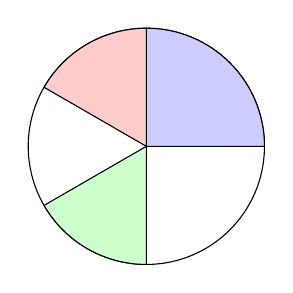
\begin{tikzpicture}
	
	\draw (0,0) circle (1.5cm);
	\filldraw[draw = black, fill=blue!20] (0,0) -- (1.5,0)  arc[radius =1.5, start angle = 0, delta angle=90] -- cycle;
	\filldraw[draw = black, fill=red!20] (0,0) -- (0,1.5)  arc[radius =1.5, start angle = 90, delta angle=60] -- cycle;
	\filldraw[draw = black, fill=green!20] (0,0) -- (0,-1.5)  arc[radius =1.5, start angle = -90, delta angle=-60] -- cycle;
\end{tikzpicture}
\end{center}
	
Exemple 1 : On fait tourner la roue ci-dessus où la flèche verte est fixe. 
Si la roue s'arrête sur une partie blanche, on gagne. 
a. Quelle est la probabilité que cela se produise ?
b. Quelle est la probabilité que l'on perde ?
a. La probabilité que la roue s'arrête en face de la flèche verte est proportionnelle à l'angle du secteur. Sachant que si l'on regarde la probabilité que : « la roue s'arrête quelque part sur le disque » est de 1 et que cela correspond à un angle de 360\degres, on peut dresser le tableau de proportionnalité suivant.
Angle
360
90
60
Et donc p(gagner) = p(blanc) =
Probabilité
1



b. L'événement : « perdre » est réalisé par les issues : « la flèche s'arrête sur le bleu, le rose ou le violet ». 
Ainsi p(perdre) = p(bleu)  p(rose)  p(violet). 
Ou encore, p(perdre)p(gagner) = 1 donc p(perdre) = 1p(gagner)



	\subsection{Exemple 2}
	
Dans une urne, il y a trois boules rouges (\textcolor{red}{R}) et deux boules bleues (\textcolor{blue}{B}). On tire successivement et avec remise deux boules. Détermine la probabilité de tirer deux boules de la même couleur.
On peut représenter cette expérience aléatoire par un tableau à double entrée.

\begin{center}
\begin{tabular}{|c|c|c|c|c|c|}
\hline
Premier tirage &  \multicolumn{5}{|c|}{Second tirage}\\
\hline
 &  \textcolor{red}{R1} & \textcolor{red}{R2} & \textcolor{red}{R3} & \textcolor{blue}{B1} & \textcolor{blue}{B2} \\
 \hline
  \textcolor{red}{R1}&  (\textcolor{red}{R1},\textcolor{red}{R1}) & (\textcolor{red}{R1},\textcolor{red}{R2}) & (\textcolor{red}{R1},\textcolor{red}{R3}) & (\textcolor{red}{R1},\textcolor{blue}{B1}) & (\textcolor{red}{R1},\textcolor{blue}{B2}) \\
 \hline
  \textcolor{red}{R2} &  (\textcolor{red}{R2},\textcolor{red}{R1}) & (\textcolor{red}{R2},\textcolor{red}{R2}) & (\textcolor{red}{R2},\textcolor{red}{R3}) & (\textcolor{red}{R2},\textcolor{blue}{B1}) & (\textcolor{red}{R2},\textcolor{blue}{B2}) \\
   \hline
    \textcolor{red}{R3} &  (\textcolor{red}{R3},\textcolor{red}{R1}) & (\textcolor{red}{R3},\textcolor{red}{R2}) & (\textcolor{red}{R3},\textcolor{red}{R3}) & (\textcolor{red}{R3},\textcolor{blue}{B1}) & (\textcolor{red}{R3},\textcolor{blue}{B2}) \\
    \hline
    \textcolor{blue}{B1} &  (\textcolor{blue}{B1},\textcolor{red}{R1}) & (\textcolor{blue}{B1},\textcolor{red}{R2}) & (\textcolor{blue}{B1},\textcolor{red}{R3}) & (\textcolor{blue}{B1},\textcolor{blue}{B1}) & (\textcolor{blue}{B1},\textcolor{blue}{B2}) \\
\hline    
    \textcolor{blue}{B2} &  (\textcolor{blue}{B2},\textcolor{red}{R1}) & (\textcolor{blue}{B2},\textcolor{red}{R2}) & (\textcolor{blue}{B2},\textcolor{red}{R3}) & (\textcolor{blue}{B2},\textcolor{blue}{B1}) & (\textcolor{blue}{B2},\textcolor{blue}{B2}) \\
\hline
\end{tabular}
\end{center}


On peut aussi dessiner un arbre de dénombrement.

\begin{center}
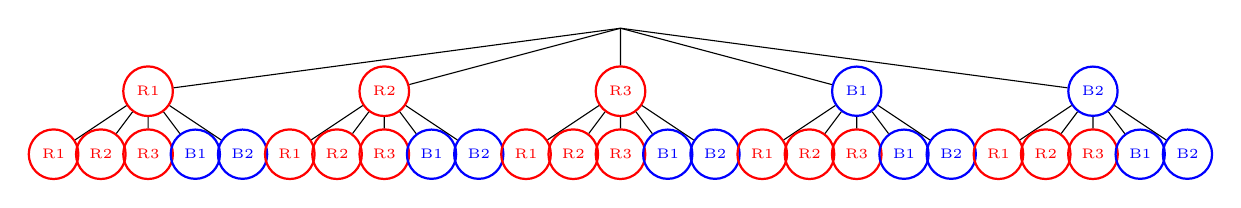
\begin{tikzpicture}
[level distance=8mm,
every node/.style={circle,draw},
level 1/.style={sibling distance = 30 mm},
level 2/.style={sibling distance = 6 mm}
]
\coordinate
child {node[thick,red] {\textcolor{red}{\tiny R1}}
child {node[thick,red] {\textcolor{red}{\tiny R1}}}
child {node[thick,red] {\textcolor{red}{\tiny R2}}}
child {node[thick,red] {\textcolor{red}{\tiny R3}}}
child {node[thick,blue] {\textcolor{blue}{\tiny B1}}}
child {node[thick,blue] {\textcolor{blue}{\tiny B2}}}
}
child {node[thick,red] {\textcolor{red}{\tiny R2}}
child {node[thick,red] {\textcolor{red}{\tiny R1}}}
child {node[thick,red] {\textcolor{red}{\tiny R2}}}
child {node[thick,red] {\textcolor{red}{\tiny R3}}}
child {node[thick,blue] {\textcolor{blue}{\tiny B1}}}
child {node[thick,blue] {\textcolor{blue}{\tiny B2}}}
}
child {node[thick,red] {\textcolor{red}{\tiny R3}}
child {node[thick,red] {\textcolor{red}{\tiny R1}}}
child {node[thick,red] {\textcolor{red}{\tiny R2}}}
child {node[thick,red] {\textcolor{red}{\tiny R3}}}
child {node[thick,blue] {\textcolor{blue}{\tiny B1}}}
child {node[thick,blue] {\textcolor{blue}{\tiny B2}}}
}
child {node[thick,blue] {\textcolor{blue}{\tiny B1}}
child {node[thick,red] {\textcolor{red}{\tiny R1}}}
child {node[thick,red] {\textcolor{red}{\tiny R2}}}
child {node[thick,red] {\textcolor{red}{\tiny R3}}}
child {node[thick,blue] {\textcolor{blue}{\tiny B1}}}
child {node[thick,blue] {\textcolor{blue}{\tiny B2}}}
}
child {node[thick,blue] {\textcolor{blue}{\tiny B2}}
child {node[thick,red] {\textcolor{red}{\tiny R1}}}
child {node[thick,red] {\textcolor{red}{\tiny R2}}}
child {node[thick,red] {\textcolor{red}{\tiny R3}}}
child {node[thick,blue] {\textcolor{blue}{\tiny B1}}}
child {node[thick,blue] {\textcolor{blue}{\tiny B2}}}
};
\end{tikzpicture}


	
\end{center}


Il y a au total 25 issues possibles. L'événement « les deux boules sont de même couleur » est réalisé par 13 issues. La probabilité d'avoir deux boules de même couleur est donc de $\dfrac{13}{25}$.

\begin{remarque}
On s'intéresse maintenant au tirage de deux boules, mais \textbf{sans} remise.\\
Dans une urne, il y a trois boules rouges (\textcolor{red}{R}) et deux boules bleues (\textcolor{blue}{B}). On tire successivement et sans remise deux boules. Détermine la probabilité de tirer deux boules de la même couleur, en dessinant un arbre de dénombrement.\\
La probabilité de cet événement est-elle la même que celle obtenue ci-dessus ?
\end{remarque}
